\documentclass[11pt]{article}

\usepackage{latexsym}
\usepackage{graphicx}
\usepackage{amssymb}
\usepackage{amsthm}
\usepackage{enumerate}
\usepackage{amsmath}
\usepackage{cancel}
\numberwithin{equation}{section}
\numberwithin{figure}{section}
\numberwithin{table}{section}

\setlength{\evensidemargin}{.25in}
\setlength{\oddsidemargin}{-.25in}
\setlength{\topmargin}{-.75in}
\setlength{\textwidth}{6.5in}
\setlength{\textheight}{9.5in}
\newcommand{\due}{April 1st, 2010}
\newcommand{\HWnum}{8}
\newcommand{\grad}{\bold\nabla}
\newcommand{\vecE}{\vec{E}}
\newcommand{\scrptR}{\vec{\mathfrak{R}}}
\newcommand{\kapa}{\frac{1}{4\pi\epsilon_0}}
\newcommand{\unit}[1]{\ensuremath{\, \mathrm{#1}}}

\begin{document}
\begin{titlepage}
\setlength{\topmargin}{1.5in}
\begin{center}
\Huge{Physics 3320} \\
\LARGE{Principles of Electricity and Magnetism II} \\
\Large{Professor Ana Maria Rey} \\[1cm]

\huge{Homework \#\HWnum}\\[0.5cm]

\large{Joe Becker} \\
\large{SID: 810-07-1484} \\
\large{\due} 

\end{center}

\end{titlepage}


\section{Introduction}
The most commonly signals in experimental physics are analog and not digital. But in order to interpret this data we need to convert the analog signal into a digital signal. Usually we use an oscilloscope to perform this action. While we do not need to understand all the inner digital circuits of the oscilloscope, it is a good idea to have a grasp of how digital circuits work. For this lab we will explore basic properties of digital circuits.

\section{Basic Logic Gate Properties}
\subsection{Theory}
In a digital circuit the signal is only in one of two states: HIGH or LOW. Where high is usually some voltage and low is usually no voltage. Generally we say that high is the logical 1 and low is the logical 0. This is a binary notation. 

The most simple logical gate is the NOT gate. This gate just inverts the input signal. So if we input a true (1) signal then the output is false (0). This gate is often called an inverter.

For this lab we look at the NAND operator. The NAND operator is a logical gate that combines the NOT and the AND operators. The symbol for the NAND gate is shown in figure \ref{FigNAND}.
\begin{figure}[h]
\centering
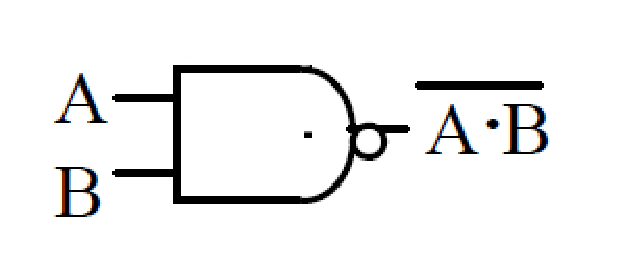
\includegraphics[scale=0.50]{FigNAND.eps}
\caption{\textit{The symbol for the NAND gate}}
\label{FigNAND}
\end{figure}
An AND gate reads two inputs and if both inputs are true (1) then the output of the AND gate is 1, otherwise the output is false (0). The NAND gate is the AND gate with a NOT gate attached, so the output of an NAND gate is the exact opposite of that for a AND gate (see the truth table for the NAND gate in table \ref{TruthTabNAND}).
\begin{table}[h]
\centering
\begin{tabular}{cc|c}
$A$	&$B$	&$\overline{A\cdot B}$\\
\hline
0	&0	&1\\
1	&0	&1\\
0	&1	&1\\
1	&1	&0\\
\end{tabular}
\caption{\textit{The truth table for the NAND gate}}
\label{TruthTabNAND}
\end{table}

Like the NAND gate the NOR gate is the inverse of the OR gate. An OR gate takes two inputs and if one or the other is true then the output is true. Note that both can be true and we will still have an output of 1. So a NOR gate is only true when both inputs are 0 (see the truth table for the NOR gate in table \ref{TruthTabNOR}). 
\begin{figure}[h]
\centering
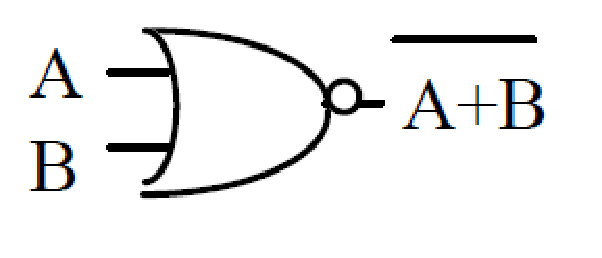
\includegraphics[scale=0.50]{FigNOR.eps}
\caption{\textit{The symbol for the NOR gate}}
\label{FigNOR}
\end{figure}
The symbol for the NOR gate is shown in figure \ref{FigNOR}
\begin{table}[h]
\centering
\begin{tabular}{cc|c}
$A$	&$B$	&$\overline{A+B}$\\
\hline
0	&0	&1\\
1	&0	&0\\
0	&1	&0\\
1	&1	&0\\
\end{tabular}
\caption{\textit{The truth table for the NOR gate}}
\label{TruthTabNOR}
\end{table}

The final logical gate we look at is th XOR gate. The XOR gate is just like the OR gate but if both $A$ and $B$ are true then the output is false (see the truth table in table \ref{TruthTabXOR}).
\begin{table}[h]
\centering
\begin{tabular}{cc|c}
$A$	&$B$	&$A\oplus B$\\
\hline
0	&0	&0\\
1	&0	&1\\
0	&1	&1\\
1	&1	&0\\
\end{tabular}
\caption{\textit{The truth table for the XOR gate}}
\label{TruthTabXOR}
\end{table}
We can make an XOR gate out of NAND, NOR, and an inverter gate (see figure \ref{FigXOR}).
\begin{figure}[h]
\centering
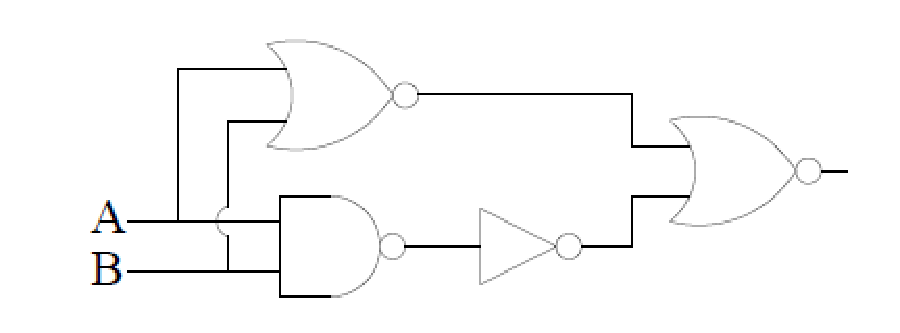
\includegraphics[scale=0.60]{FigXOR.eps}
\caption{\textit{An XOR gate constructed from NAND and NOR gates. Note that the triangle symbol is the inverter.}}
\label{FigXOR}
\end{figure}
Note that we inverting the output of a NOR gate is the same as an OR gate. 

\subsection{Experiment}
For this experiment we used the DC power supply and sent to the breadboard $+5\unit{V}$. We used a 10 LED bar to test the output of the logic gates where on was true and off was false. First we tested to make sure that the LEDs were functional. Next connected the output of the NAND (7400) IC to the LED and verified that the truth table in table \ref{TruthTabNAND} was correct. We then tested the NOR (7402) IC in the same way, again we verified that table \ref{TruthTabNOR} was valid. 

To test the XOR gate we used build the logical gate shown in figure \ref{FigXOR} using the NAND IC and the NOR IC. Note that we used the inverter IC (7404). Again we found that table \ref{TruthTabXOR} was correct. 

\section{RS Flip-Flop}
\subsection{Theory}
The RS Flip-Flop is a circuit constructed by two NOR gates (see figure \ref{FigRSFlipFlop}). 
\begin{figure}[h]
\centering
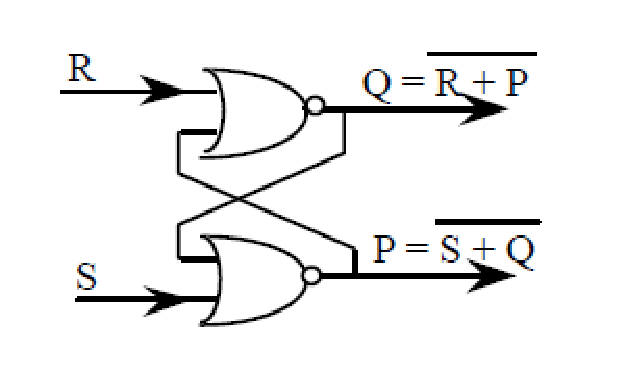
\includegraphics[scale=0.60]{FigRSFlipFlop.eps}
\caption{\textit{The RS Flip-Flop constructed from two NOR gates.}}
\label{FigRSFlipFlop}
\end{figure}
The unique property of the RS Flip-Flop is that it can store the value. The $S$ input ($S$ is for set) will set the output $Q$ to that value. So if $S=1$ and $R=0$ then $Q=1$, the important part to note is that $Q$ remains true even after $S$ and $R$ are both false. The opposite case is valid as well, if $S=0$ and $R=1$ then $Q=0$, and $Q$ will remain false when both $S$ and $R$ are false. Note that $S=R=1$ is a disallowed input for this circuit and will have both $P$ and $Q$ be false even though $P=\overline{Q}$. See the truth table for the RS Flip-Flop in table \ref{TruthTabRS}
\begin{table}[h]
\centering
\begin{tabular}{cc|cc}
$S$	&$R$	&$Q$	&$P=\overline{Q}$\\
\hline
1	&0	&1	&0\\
0	&1	&0	&1\\
\hline
0	&0	&\multicolumn{2}{c}{Stays the same}
\end{tabular}
\caption{\textit{The truth table for the RS Flip-Flop. Note that for $R=S=0$ we recall the stored value for $Q$.}}
\label{TruthTabRS}
\end{table}

\subsection{Experiment}
For this part we constructed the RS Flip-Flop using two NOR gates as shown in figure \ref{FigRSFlipFlop}. Note that we still have $+5\unit{V}$ DC running into th circuit. We connected the output of the RS Flip-Flop to the 10 LED bar. We then set $Q=1$ by setting $S=1$ and $R=0$. Then we set both $R$ and $S$ to false and noted that the LED remained on. We did the same for $Q=0$ and found that $Q$ remained false. Thus the truth table in table \ref{TruthTabRS} is valid.

\section{TTL Clock}
\subsection{Theory}
We can use a 555 timer to make a clock. For our purposes we by clock we mean a circuit that pulse at a high voltage for some time $T_2$ then drops to a lower voltage for some time $T_1$. 
\begin{figure}[h]
\centering
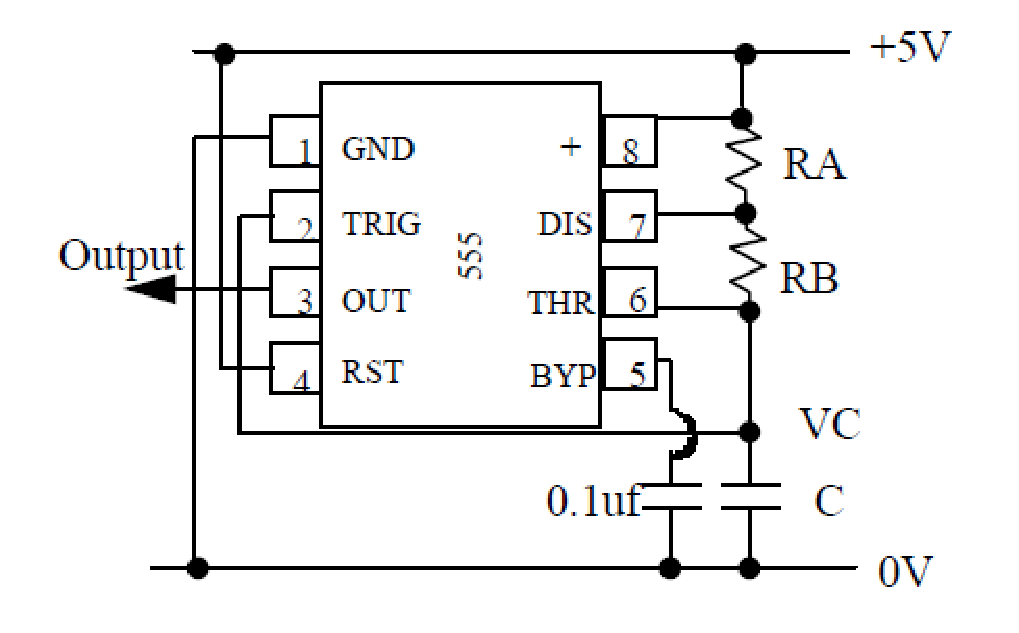
\includegraphics[scale=0.50]{Fig555Timer.eps}
\caption{\textit{The schematic for the 555 timer clock.}}
\label{Fig555Timer}
\end{figure}
To do this we use a 555 timer and a capacitor as shown in figure \ref{Fig555Timer}. Note that the period of the clock is given by the sum $T = T_1+T_2$. Where $T_1$ and $T_2$ are determined by the resistors $R_A$ and $R_B$ and the capacitor $C$ by 
\begin{equation}
T_1 = R_BC\ln(2)
\label{Time1}
\end{equation}
\begin{equation}
T_2 = (R_A+R_B)C\ln(2)
\label{Time2}
\end{equation}

\subsection{Experiment}
We built the circuit in figure \ref{Fig555Timer} where $R_A = 678\unit{k\Omega}$ and $R_B = 320\unit{k\Omega}$ and a capacitor $C=1.00\unit{nF}$. We then connected the output of this circuit to the oscilloscope using the 10$\times$ probe. We measured the amplitude of the output as $4.70\unit{V}$. Note that the low pulse was at $0\unit{V}$ and the high pulse was at $4.70\unit{V}$. Then we measured the time of each pulse using the cursors on the oscilloscope. We measured that $T_1 = 496\unit{\mu s}$ and $T_2 = 720\unit{\mu s}$. Using equations \ref{Time1} and \ref{Time2} and the values we measured for $R_A$, $R_B$, and $C$ we expect that $T_1 = 222\unit{\mu s}$ and $T_2 = 690\unit{\mu s}$. Note that the measured value for $T_2$ is close to the value we expected. But the measure value for $T_1$ is longer than we expect. This is due to the capacitor taking a longer time to discharge, this could be due to internal inductances and capacitances.

Next to test that the period will drop to $1\unit{Hz}$ we removed the $1.00\unit{nF}$ capacitor and replaced it with a $33\unit{nF}$ capacitor. We noticed that the period dropped to about $1\unit{Hz}$ as we expected.

\section{JK Flip-Flop}
\subsection{Theory}
A JK Flip-Flop has 4 inputs $J$ and $K$ are the user controlled inputs, where $C$ is the clock input that drives the IC and $CLR$ is the clear input. See figure \ref{FigJKFlipFlop}.
\begin{figure}[h]
\centering
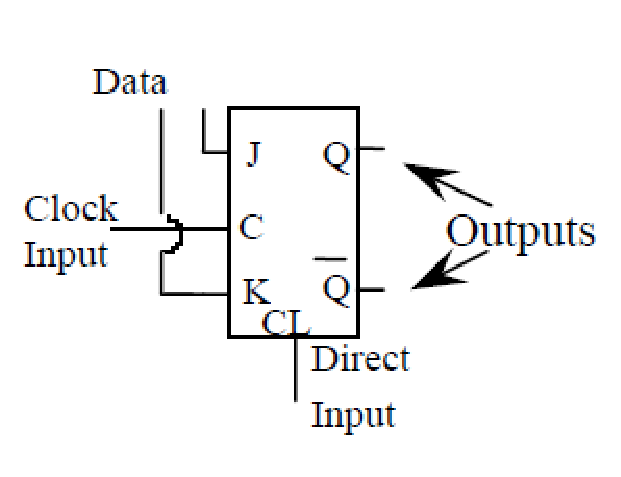
\includegraphics[scale=0.60]{FigJKFlipFlop.eps}
\caption{\textit{The symbol for the JK Flip-Flop.}}
\label{FigJKFlipFlop}
\end{figure}

\begin{table}[h]
\centering
\begin{tabular}{c|cc|cc}
$CLR$	&$J$	&$K$	&$Q_{n+1}$		&$\overline{Q_{n+1}}$\\
\hline
1	&0	&0	&$Q_n$			&$\overline{Q_n}$\\
1	&1	&0	&1			&0\\
1	&0	&1	&0			&1\\
1	&1	&1	&$\overline{Q_n}$	&$Q_n$\\
\hline
0	&\multicolumn{2}{c}{Anything}	&0	&1
\end{tabular}
\caption{\textit{The truth table for the JK Flip-Flop.}}
\label{TruthTabJK}
\end{table}
The JK Flip-Flop works much like the RS Flip-Flop where $J$ is the set and $K$ is the reset. So when we have $J=1$ and $K=0$ we set the output $Q$ to be true. And if we set $J$ to false and $K$ to true we set $Q=1$. Note like the RS Flip-Flop $J=K=0$ will recall the saved value for $Q$, but for the JK Flip-Flop $J=K=1$ will give the inverse of the output or $\overline{Q}$. Note that the $CLR$ input has to be set to true for this to work. If $CLR$ is false then $Q$ is always false, this is why the $CLR$ is the clear input. See the truth table for the JK Flip-Flop in table \ref{TruthTabJK}.

\subsection{Experiment}
To begin we made the circuit shown in figure \ref{FigSchemJKFlipFlop}.
\begin{figure}[h]
\centering
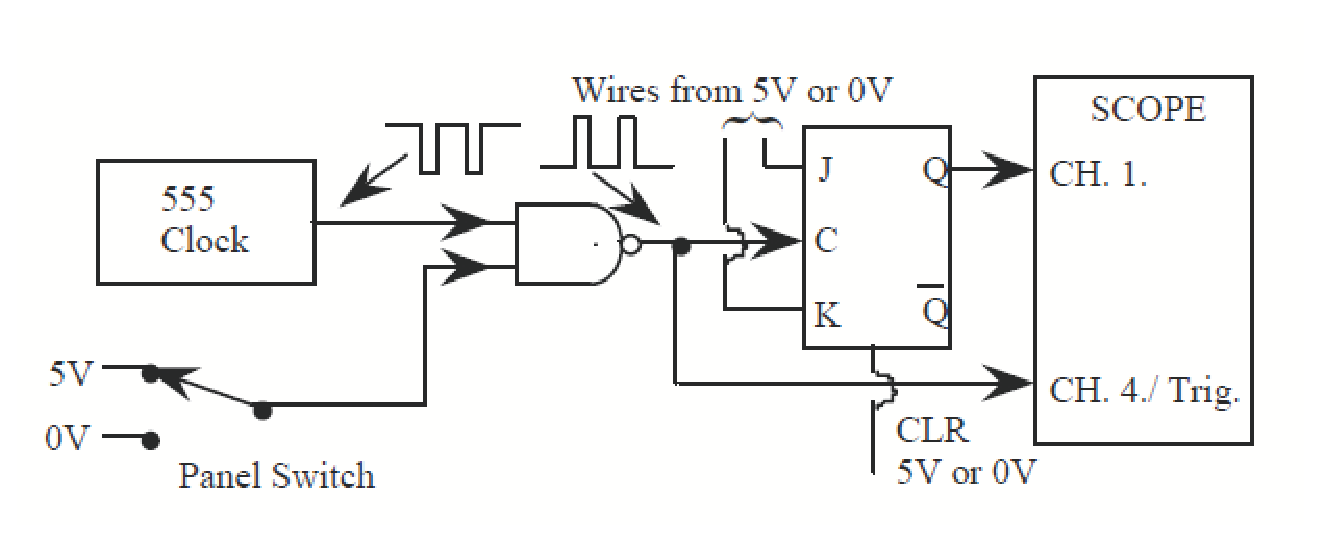
\includegraphics[scale=0.60]{FigSchemJKFlipFlop.eps}
\caption{\textit{The schematic for the circuit we built to test the JK Flip-Flop. Note that the 555 timer clock was the same as we used before.}}
\label{FigSchemJKFlipFlop}
\end{figure}
We used the 555 timer clock described in figure \ref{Fig555Timer} and a NAND gate to make the output more digital. We then tested the truth table in table \ref{TruthTabJK}. We confirmed that the truth table is valid.

Next we connected the output from the clock (after it passes through the NAND gate) and the output from the JK Flip-Flip. We then set $J=K=1$ and we noted how the output $Q$ changes with each period of the clock. Attached is the waveforms from the oscilloscope. Then we set $J=K=0$ this time the output $Q$ was at a constant $1$ as we expected. Note that there a aberrations every period of the clock. This happened in both cases so we determined that the effect can be ignored.

\section{Conclusion}
Digital circuits are important to everyday life. We found using Flip-Flops that simple logical gates can be used to store a bit of data. This is the foundation of digital electronics.
\end{document}

